\section{What the model implies}\label{sec:results}

The paper draws its results in four steps: topic choice without an entry cost, topic choice with one, the effect of tools, and what happens to topics over time.

\subsection{Free topic choice without an entry cost}

Set $b_c=\infty$, so newcomers pay nothing to get in and $w=v$.

\begin{resultbox}{Proposition 2}{Equilibrium and dissipation}{\tsolid}
A topic equilibrium exists and is unique. Every open topic sits on the \emph{falling} side of the payoff curve, $P^*>\Phat$. Output per researcher equals the frontier value, $aF<a\vhat$: the gain from cumulative knowledge, $\vhat-F$, is competed away. With founders who stay and no depletion, density solves $v(P^*)=e$ whatever the founders' share.
\tcblower
\inwords A newcomer compares the \emph{average} payoff in a topic with the frontier. She ignores that her papers lower everyone else's payoff once the topic is past its peak. So topics fill past the peak, until being inside is no better than exploring.

\why Crossings on the rising side are unstable: one more entrant raises the payoff of entering.

\review Correct as a benchmark (here Lemma~4 holds exactly). It is the theory of city sizes of Henderson (1974) and of clubs of Buchanan (1965), and the paper says so. What is specific to topics: the hump is derived, the congestion is in attention (``the crowders are the readers''), and the duplication rate depends on density alone. Its implication of equal returns across topics is rejected by Fact~2, which is why the entry cost is added.
\end{resultbox}

\begin{resultbox}{Proposition 3}{Volume opens new topics}{\tsolid}
In the large-topic limit, equilibrium density depends on the number of researchers and on production speed only through the product $Na$, and
\[
\EE\equiv\frac{\dd\ln P^*}{\dd\ln N}=\frac{\etaF}{\etaF D+|\eps_w|+\thF\,\eps_U},\qquad D\ge 1,
\]
where $\eps_w<0$ is the elasticity of the newcomer's payoff with respect to density and $\eps_U$ that of the founder's payoff. New topics absorb a share $1-D\EE$ of growth. If the frontier is not depleted ($\etaF=0$), density, the overlap rate and the aware share do not depend on $N$, on $a$, or on the cost of entering science.
\tcblower
\inwords When the community grows, the extra researchers open new topics until the existing ones are no more attractive than the frontier. Topics get denser only to the extent that good new topics become harder to find. A fixed idea space is the opposite extreme ($\etaF\to\infty$): all growth thickens existing topics.

\role This is where the theory meets the data. Fact~1 measures $\EE$ at 0.12--0.19 against 0.53--0.81 for a fixed idea space. Inverting the formula gives the depletion of the frontier, $\etaF=\EE(|\eps_w|+\thF\eps_U)/(1-\EE D)$. The paper also notes (Remark~4) that mature topics adjust to more researchers \emph{at once}, because the marginal newcomer is indifferent.

\review The algebra is right, and this is the best-supported result in the paper. Two caveats. The formula contains the unmeasured $\thF$, so it should be used to interpret $\EE$, not to derive numbers. And ``only through $Na$'' is a statement about the long run: in the short run more researchers and faster researchers are absorbed very differently, which the paper has in an appendix and which Part~III makes the main idea (\S\ref{sec:ideas-scale}).
\end{resultbox}

\begin{resultbox}{Proposition 4}{Overcrowding and the frontier subsidy}{\trepair}
(i)~Output per researcher at a common density is $a\,w(P)$, so a planner puts every topic at the peak of the newcomer's payoff, $\hat P_w$; she opens more topics with fewer researchers in each. The gain is $\hat w/F-1$.
(ii)~Counting explorers, the planner's density lies between $\hat P_w$ and $P^*$.
(iii)~A subsidy to the frontier (or a tax on joining open topics) of $\hat w-F$ decentralises the optimum.
(iv)~There are two wedges, a \emph{crowding wedge} (newcomers use the average payoff, the planner the marginal one) and a \emph{production wedge} (researchers ignore that their papers add to what colleagues must read). The second vanishes at the optimal density.
\tcblower
\inwords Topics are too crowded and there are too few of them. Fix the allocation of people to topics and the way they split their time takes care of itself.

\review The direction is robust; the size is not. The proof switches between two exponents for the share of members who produce. The planner's gain is 1.25\% under one and 0.37\% under the other, and 0.5--1.0\% once explorers are counted. All are small (\S\ref{sec:crit-lemma4}).
\end{resultbox}

\begin{figure}[h]
\centering
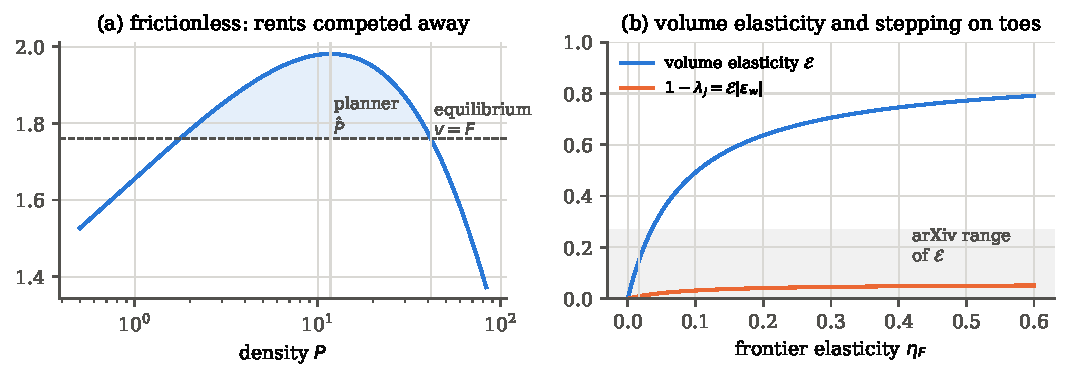
\includegraphics[width=0.98\textwidth]{fig2_planner_volume.pdf}
\caption{From the paper (its Figure~2). Left: without an entry cost topics fill to the density where $v=F$; the shaded rent is competed away and the planner puts topics at the peak. Right: the volume elasticity $\EE$ as a function of the depletion of the frontier; the shaded band is the range of arXiv estimates.}
\end{figure}

\subsection{Topic choice with an entry cost: rents and the speed limit}

Now $b_c<\infty$. Newcomers must read a topic's stock before they contribute.

\begin{resultbox}{Proposition 5}{Mature topics under catch-up costs}{\tsolid}
(i)~The newcomer's payoff $w(P)=v(P)(1-P/b_c)^{\nu}$ has a single peak $\hat P_w$, below the peak of $v$, and vanishes at $b_c$.
(ii)~The mature density $\Pm$ solves $w(\Pm)=F$ on the falling side of $w$. Incumbents earn a premium over the frontier equal to the catch-up cost:
\[
\ln\frac{v(\Pm)}{F}=(\rho+\xi)\,T(\Pm).
\]
(iii)~Mature topics lie on the \emph{rising} side of $v$ when catch-up is costly relative to the rent at the peak.
(iv)~If topics differ in fertility, then across mature topics log returns rise with log density at the catch-up elasticity
$\eps_\Gamma(\Pm)=\nu\,\dfrac{\Pm/b_c}{1-\Pm/b_c}$, which exceeds the premium.
\tcblower
\inwords The entry cost turns the rent that was competed away into a protected one. Insiders earn more than the frontier, by exactly what a newcomer gives up while she reads her way in. More fertile topics attract more people, build larger literatures and protect larger premia. So returns rise with density across topics.

\review Rederived and correct. These results need neither the speed limit, nor the founders' assumption, nor Lemma~4. They are the distinctive, reliable core of the catch-up block. In the calibration the premium is 10.3\% (a catch-up time of 0.74 years) and the gradient is 0.113. The measured gradient (6.7\% per standard deviation) is an upper bound on it, because citations also reward audience.
\end{resultbox}

\begin{resultbox}{Corollary 1}{Overcrowding with rising returns}{\tsolid}
In every stable equilibrium one more member lowers the total output of the others, counting both the spillover on incumbents ($v'$) and the extra reading she imposes on future newcomers ($v\Gamma'$). If $w(\Phat)<F$ then $\hat P_w<\Pm<\Phat$: incumbents' returns \emph{rise} with density ($v'>0$) while the topic is \emph{too crowded} ($w'<0$).
\tcblower
\inwords The data show that the same researcher earns more in denser topics. The natural reading is that topics are too thin. The corollary says that this confuses what an insider earns with what a newcomer can expect. Rising returns are the footprint of an entry barrier, not of an untapped spillover.

\review The sign statement is solid and worth keeping: it is the reason incumbents stay and newcomers go elsewhere. The welfare magnitude attached to it shares the accounting problem of Proposition~4.
\end{resultbox}

\begin{resultbox}{Theorem 2}{The speed limit}{\tinert}
(i)~\emph{Closure.} A topic whose flow is at least $b_c$ is closed: anyone who joins never catches up.
(ii)~\emph{Rents near the limit.} Every mature topic has $\Pm<b_c$. As fertility rises, $\Pm\to b_c$ and both the premium and the returns gradient grow without bound.
(iii)~\emph{Growing topics.} Myopic entry into a growing topic stops before its flow reaches $b_c$.
(iv)~\emph{Production shocks.} A speed-up of production by a factor $1+\alpha$ raises every topic's flow by that factor on impact. Every topic with $\Pm>b_c/(1+\alpha)$ closes and stays closed for at least $\ln[(1+\alpha)\Pm/b_c]/\rho$ periods.
\tcblower
\inwords A literature can grow faster than outsiders can absorb it. When it does, the topic is shut however rewarding it is inside. A tool that lets everyone produce faster pushes the densest topics past the limit for a while.

\review Correct mathematics that never operates. In the calibrated economy the typical mature topic is at 17\% of the limit, the most fertile at 33\%, and no researcher-year is above 53\%. Closing the densest topic needs production to triple. The limit exists only because newcomers must read \emph{everything} while insiders read a third of the flow. Part~(iii) fails with forward-looking entry. A cost with no limit fits the data equally well (\S\ref{sec:crit-speed}). Part~(iv) is the useful piece: it is the seed of the scale-versus-speed idea.
\end{resultbox}

\paragraph{Newborn topics (Remark 6)} A newborn topic has no stock, so its first follower needs no catch-up and earns $v(P_0)$, where $P_0$ is the flow of a newborn topic. New topics attract followers only if $v(P_0)>F$. In the calibration $v(P_0)>F>w(P_0)$: a newborn topic is worth joining while its stock is empty, but a stationary topic of the same density is not. This is the starting point of the life-cycle results below.

\begin{resultbox}{Proposition 6}{Social value and priority transfers}{\tminor}
Part of the credit a duplicate loses is a transfer to the earlier paper. If a share $\tau$ of overlap losses is a transfer, the equilibrium is still overcrowded as long as $\tau<|\eps_w(\Pm)|/(\theta\lambda\Pm)$.
\tcblower
\inwords The welfare results count private credit, and priority credit is partly redistribution. This does not reverse the result, because the reading that newcomers impose on one another is a real cost. In the calibration the critical transfer share is above one. The planner's gain shrinks from 1.2\% to 0.4\% if all overlap losses are transfers.

\review Correct. Not mentioned in the introduction, and nothing else depends on it.
\end{resultbox}

\subsection{Tools}\label{sec:results-tools}

A tool enters the model through one of its parameters: production speed $a$, reading speed $b$, learning $\beta$, search precision $\sigma$, the cost of pivoting $\kappa_p$, catch-up speed $b_c$, or the cost of entering science. Lemma~5 prices each inside a topic. The question of this section is where that value ends up once researchers move.

\begin{resultbox}{Theorem 3}{Frontier incidence}{\trepair}
Let a tool raise the newcomer's payoff $\ln w$ by $h$ and the frontier value $\ln F$ by $f$ at a given density. Then
\begin{gather*}
\dd\ln\frac{Y}{N}=\dd\ln a+\lambda_F\,f+(1-\lambda_F)\,h,\qquad
\dd\ln P^*=\frac{h-f}{\Psi},\\
\lambda_F=\frac{|\eps_w|}{\Psi},\qquad \Psi=|\eps_w|+\thF\,\eps_U+\etaF D .
\end{gather*}
The share of a newcomer-side gain that survives entry is
\[
1-\lambda_F=1-(1-\EE D)\,\frac{|\eps_w|}{|\eps_w|+\thF\,\eps_v}\ \ge\ \EE D .
\]
\tcblower
\inwords In the long run a tool is worth what it adds to the value of opening a new topic. A tool that raises payoffs only inside existing topics draws newcomers in until those topics are again no better than the frontier. Its gain survives only through two channels: founders who stay earn the payoffs of the denser topics they end up in ($\thF$), and fewer topics leave better directions open ($\etaF$). The data put a floor under the surviving share: the volume elasticity.

\review The algebra is right as a statement about the frontier value and about density. The step to output per researcher uses Lemma~4 and fails. Repaired, the theorem has a third channel: members who entered before entry was costly keep their gain too. The numbers move from 14--74\% to 53--88\% (\S\ref{sec:crit-lemma4}). Structurally it is the free-entry incidence result of spatial economics; the application to research tools is new (\S\ref{sec:crit-novelty}).
\end{resultbox}

\begin{resultbox}{Corollary 2}{Ranking tools}{\tassumed}
(i)~\emph{Production tools} act like a larger community: $\dd\ln(Y/N)/\dd\ln a=1-\EE|\eps_w|$, about 0.99.
(ii)~\emph{Learning tools} (reading, learning, search, pivots) raise $v$ at every density. Founders read too, so a share $\Pi_L=1-\lambda_F(1-\thF)$ survives.
(iii)~\emph{Catch-up tools} raise only newcomers' payoffs. Founders never catch up, so a share $\Pi_C=1-\lambda_F$ survives.
(iv)~Hence $\Pi_C\le\Pi_L\le 1-\EE|\eps_w|$.
\tcblower
\inwords Tools that help the people who open topics keep their value. Tools that help only the people who join topics lose most of it.

\review The ordering follows from what explorers are assumed to do: their output scales with production speed and with nothing else, they found topics without reading, and new topics are as fertile as old ones. With the fertility depletion of the paper's own Appendix~B.1 the ranking of production over reading reverses (\S\ref{sec:crit-ranking}). The honest statement is an accounting of where gains go, not a ranking.
\end{resultbox}

\begin{center}\small
\begin{tabularx}{\textwidth}{@{}Lrrrrr@{}}
\toprule
 & \multicolumn{3}{c}{Output per researcher (log points)} & \multicolumn{2}{c}{Footprints ($\omega=\tfrac12$)} \\
\cmidrule(lr){2-4}\cmidrule(l){5-6}
Tool, 30\% better & Fixed topics & Long run, $\omega=0$ & Long run, $\omega=\tfrac12$ & Density & Topics \\
\midrule
Faster production ($a$) & $+26.2$ & $+26.0$ & $+26.0$ & $+3.8$ & $+22.0$ \\
Faster reading ($b$) & $+2.0$ & $+0.3$ & $+1.5$ & $+7.8$ & $-8.0$ \\
Better learning ($\beta$) & $+4.1$ & $+0.5$ & $+2.9$ & $+14.6$ & $-16.3$ \\
Better search ($\sigma$) & $+0.1$ & $+0.0$ & $+0.1$ & $+0.5$ & $-0.4$ \\
Cheaper pivots ($\kappa_p$ halved) & $+0.6$ & $+0.1$ & $+0.5$ & $+2.5$ & $-3.0$ \\
Faster catch-up ($b_c$) & $+2.6$ & $+0.4$ & $+1.0$ & $+26.3$ & $-27.1$ \\
\bottomrule
\end{tabularx}
\par\smallskip
\parbox{\textwidth}{\footnotesize The paper's Table~2, abridged. $\omega$ is the share of an explorer's time spent as the founder of a topic; the paper sets it to one half by assumption. These are the numbers \emph{as the paper reports them}; \S\ref{sec:crit-lemma4} gives the corrected ones.}
\end{center}

\begin{resultbox}{Proposition 7}{Footprints of new research tools}{\tuntested}
(i)~Faster production: density moves with elasticity $\EE$, the number of topics with $1-D\EE$, papers per researcher rise about one for one.
(ii)~Cheaper entry into science raises $N$, with the effects of Proposition~3.
(iii)~Better reading, learning or search, or cheaper pivots: density rises and the number of topics falls. \emph{Science concentrates.}
(iv)~Faster catch-up: the same, more strongly; it also raises the speed limit and makes overshooting more common.
(v)~Better search raises the aware share.
\tcblower
\inwords Each kind of tool leaves a different trace in observables. Reading and catch-up tools pull people into existing topics; production tools do not.

\review Nothing tests it. The only evidence offered, for part~(i), is the ``$+7\%$'' for adopters of language models, which is a pre-existing trend (\S\ref{sec:crit-evidence}).
\end{resultbox}

\begin{resultbox}{Proposition 8}{Valuing output by readership}{\tminor}
Reads per paper are $\mathcal A=(b/a)\,r^*/(1-r^*)$. If output is valued as $\mathcal A^{\alpha}Y$, a production tool adds about nothing at $\alpha=1$ and a reading tool adds about $\dd\ln b$. The ranking of Corollary~2 reverses.
\tcblower
\inwords Total reading is fixed by researchers' time. A faster pen spreads it over more papers, so each paper is read less. A 30\% production tool lowers reads per paper by about a quarter. If science values papers by how much they are read, only reading tools raise output.

\review The reversal is built into the unit: by definition $\mathcal A$ rises one for one with $b$ and falls one for one with $a$. There is no foundation for why doubling reading speed should double the value of science, so the paper reports a ranking and its reversal without a criterion to choose between them. It also omits catch-up reading, which is 29\% of all reads in a mature topic. The thought behind it is the literal meaning of the title, and it deserves a model of its own (\S\ref{sec:ideas-other}).
\end{resultbox}

\subsection{Topics over time, growth and policy}

\begin{resultbox}{Proposition 9}{Too slow and too fast}{\tfragile}
A topic is born with flow $P_0$ and an empty stock, and grows at an exogenous diffusion rate $g$ while entry pays. The stock lags the flow: $S(P)<P/(g+\delta)$.
(i)~\emph{Take-off.} If $w(P_0)<F<v(P_0)$ there is a threshold $g_0$: topics that grow more slowly stall before they are worth joining and are abandoned.
(ii)~\emph{Overshooting.} A topic overshoots the peak of $v$ if and only if $g>g^*=\max\{g_0,g_{\hat P}\}$, with a closed-form bound.
(iii)~\emph{Foresight.} Overshooting survives when newcomers correctly anticipate the topic's path, above a threshold $g^*_{RE}$.
(iv)~\emph{Consolidation.} After entry stops incumbents stay, and the topic thins at rate $\rho$.
\tcblower
\inwords A fast-growing topic has a small literature relative to its current size, so it is cheap to join. People pile in, and the topic ends up larger than is good for it. The reading comes later, for the people who arrive later. A slow topic has the opposite problem: its literature catches up with it before it is big enough to be worth joining.

\review The stock--flow lag is the most original mechanism in the draft. As written it is fragile. Two steps of the proof are verified only numerically (both have short proofs). The take-off threshold exists only for a birth flow between 1.76 and 2.68 papers a year, and 2 is assumed; in the calibration no topic stalls for slow growth. And the law of motion omits the catch-up delay: entrants add to the flow the day they arrive (\S\ref{sec:crit-dynamics}). In the calibration the thresholds are 2.2\% a year for take-off and 20.5\% for overshooting (24.0\% with foresight).
\end{resultbox}

\begin{figure}[h]
\centering
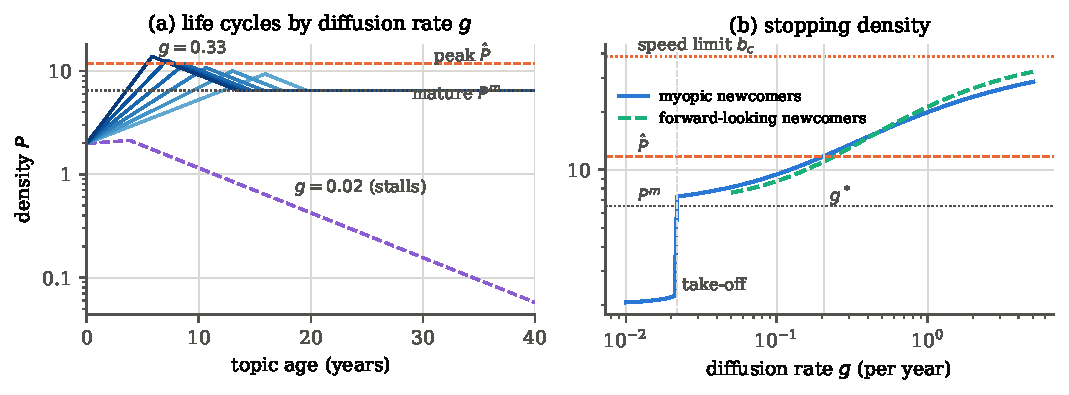
\includegraphics[width=0.98\textwidth]{fig3_lifecycle.pdf}
\caption{From the paper (its Figure~7). Left: density paths of topics with different diffusion rates. A slow topic stalls and is abandoned (dashed); fast ones overshoot the peak and thin slowly. Right: the density at which entry stops, for myopic and forward-looking newcomers.}
\end{figure}

\begin{resultbox}{Proposition 10}{Stepping on toes}{\tfragile}
With $Y=NaF$: \quad $\lambda_J^{\rm eq}=\dd\ln Y/\dd\ln N=1-\EE|\eps_w|$ when topics adjust, and $\lambda_J^{M}=1+\eps_w/D$ when the open topics are held fixed.
\tcblower
\inwords Growth models let ideas scale with researchers as $N^{\lambda_J}$ with $\lambda_J<1$ (``stepping on toes''). Here the parameter is built from two observables. In the calibration it is 0.990 (0.941 with topics fixed): crowding of topics explains little of the measured decline in research productivity.

\review The proof uses Lemma~4, and the number assumes that new topics are as fertile as old ones. With fertility depletion it is an upper bound. It is 0.98--1.00 across every calibration tried, but only because all of them set that depletion to zero.
\end{resultbox}

\begin{resultbox}{Proposition 11}{Policy that depends on a topic's age}{\tfragile}
(i)~A flat subsidy to exploring larger than $v(P_0)-F$ deters the first follower of every newborn topic. No topic then takes off.
(ii)~An entry tax proportional to the stock a newcomer must read is zero in a newborn topic, and with rate $\tau^o=\delta(\hat w-F)/\hat P_w$ it puts mature topics at the peak of $w$.
\tcblower
\inwords The textbook remedy, subsidise the frontier, backfires for young topics: it raises the bar for the people who carry a new topic through its first years. A tax that grows with a topic's literature does not. In practice: reward contributions to young topics more than contributions to old, crowded ones.

\review ``The stationary subsidy (1.25\%) is almost as large as the newborn margin (1.28\%)'' is an artefact of the assumed birth flow and of where the parameter search stopped. Only the ranking survives: the stock tax beats the flat subsidy by a factor of 2 to 5.6, with gains of 0.13--0.72\% of output.
\end{resultbox}

\subsection{The eight extensions of Appendix B}

{\small
\begin{longtable}{@{}P{0.35in}P{1.6in}P{3.75in}@{}}
\toprule
 & Extension & What it shows \\
\midrule
\endhead
\bottomrule
\endfoot
B.1 & Fertility depletion (Proposition 12) & Later topics may be less fertile, at elasticity $\eta_f$. Density data identify only the depletion of \emph{access}, not of fertility. Output per researcher then falls with the number of topics. \textbf{This extension reverses the ranking of tools.} \\
B.2 & Fertility differences & More fertile topics are denser and closer to the speed limit; infertile ones are abandoned. \\
B.3 & Nested topics (Proposition 13) & Topics inside fields give the pattern of Fact~1: close neighbourhoods are pinned, broad ones fill. Two free parameters for two elasticities, so a measurement and not a test. \\
B.4 & Learning from the stock & Stationary results are unchanged. Newborn topics attract followers only if at most 11\% of learning draws on the stock. \\
B.5 & Search on every project (Proposition 14) & If the search for overlap is repeated for every project, production speed no longer drops out of the payoff curve, and faster production lowers search per project. \\
B.6 & Differences in ability & Sorting of able researchers into dense topics could explain part of the returns gradient. Left for future work. \\
B.7 & Credit rules & Only three combinations of the credit parameters matter. \\
B.8 & A production shock over time & Every topic's flow jumps at once, newcomers go to the frontier, topics thin through turnover. \textbf{The seed of the idea in \S\ref{sec:ideas-scale}}, and wrong in two details. \\
\end{longtable}
}

\begin{keybox}[What the theory adds up to]
Without an entry cost, topics fill until nobody gains from being inside (Proposition~2), and growth opens new topics (Proposition~3).
With an entry cost, insiders keep a rent (Proposition~5) and returns rise with crowding in topics that are too crowded (Corollary~1).
A tool is worth the time it saves inside a topic (Lemma~5); after entry, what is left of it is what reaches the frontier (Theorem~3).
Fast-growing topics overshoot because the literature a newcomer must read lags behind (Proposition~9).
\end{keybox}
